\documentclass[aspectratio=169,11pt]{beamer}

\usepackage[T1]{fontenc}
\usepackage{lmodern}
\usepackage{amsmath,amssymb}
\usepackage{booktabs}
\usepackage{array}
\newcolumntype{L}[1]{>{\raggedright\arraybackslash}p{#1}}
\usepackage{tikz}
\usetikzlibrary{positioning,arrows.meta}

% Colors (same blue as the report)
\definecolor{customblue}{RGB}{0,102,204}
\definecolor{softblue}{RGB}{232,241,251}
\definecolor{ink}{RGB}{33,37,41}
\definecolor{muted}{RGB}{108,117,125}
\definecolor{m1}{RGB}{42,120,214}
\definecolor{m2}{RGB}{235,104,52}
\definecolor{m3}{RGB}{27,175,122}

% Minimal theme
\usefonttheme{professionalfonts}
\setbeamertemplate{navigation symbols}{}
\setbeamercolor{normal text}{fg=ink,bg=white}
\setbeamercolor{frametitle}{fg=customblue,bg=white}
\setbeamercolor{title}{fg=customblue}
\setbeamercolor{structure}{fg=customblue}
\setbeamercolor{block title}{fg=white,bg=customblue}
\setbeamercolor{block body}{fg=ink,bg=softblue}
\setbeamerfont{frametitle}{series=\bfseries,size=\Large}
\setbeamertemplate{itemize items}{\color{customblue}\textbullet}
\setbeamertemplate{blocks}[rounded]
\setbeamertemplate{frametitle}{\vspace{0.5em}\insertframetitle\par\vspace{-0.2em}{\color{customblue!30}\rule{\textwidth}{0.6pt}}}
\setbeamertemplate{footline}{%
  \hspace{1.2em}{\color{muted}\scriptsize KerSplit\quad\textbullet\quad\insertsection}%
  \hfill{\color{muted}\scriptsize\insertframenumber\,/\,\inserttotalframenumber}\hspace{1.2em}\vspace{0.8em}}

\tikzset{
  box/.style={draw=#1, line width=1.2pt, rounded corners=4pt, fill=#1!8,
              minimum width=2.2cm, minimum height=1.35cm, align=center, font=\small},
  arr/.style={-{Stealth[length=6pt]}, line width=1pt, color=muted}}

\newcommand{\Zp}{\mathbb{Z}_p}
\newcommand{\Zpx}{\mathbb{Z}_p[x]}
\newcommand{\aside}[1]{{\color{muted}\small #1}}

% A section opener: big title, presenter, colored bar
\newcommand{\partslide}[3]{%
  \section{#2}
  \begin{frame}[plain]
    \vfill
    {\color{#1}\rule{3em}{4pt}}\par\vspace{0.6em}
    {\color{muted}\large #3}\par\vspace{0.3em}
    {\Huge\bfseries #2}
    \vfill
  \end{frame}}

\title{KerSplit}
\subtitle{Factoring polynomials over $\mathbb{Z}_p$ with Berlekamp's algorithm}
\author{Arjun Konidala \and Sai Deepak \and Ram Panikar}
\institute{CS5610 Computational Number Theory and Algebra, IIT Hyderabad}
\date{November 2026}

\begin{document}

% -------------------------------------------------------------------------
\section{Introduction}

\begin{frame}[plain]
  \vfill
  {\color{customblue}\rule{3em}{4pt}}\par\vspace{0.8em}
  {\fontsize{40}{44}\selectfont\bfseries\color{customblue} KerSplit}\par\vspace{0.4em}
  {\Large Factoring polynomials over $\mathbb{Z}_p$ with Berlekamp's algorithm}\par\vspace{1.6em}
  {\color{ink} Arjun Konidala \quad\textbullet\quad Sai Deepak \quad\textbullet\quad Ram Panikar}\par\vspace{0.3em}
  {\color{muted}\small CS5610 Computational Number Theory and Algebra, IIT Hyderabad, November 2026}
  \vfill
\end{frame}

\begin{frame}{The problem}
  \begin{columns}[T]
    \begin{column}{0.48\textwidth}
      \textbf{Input:} a prime $p$ and $f \in \Zpx$ of degree $d$\par\medskip
      \textbf{Output:}
      \[ f = c \cdot h_1^{e_1} h_2^{e_2} \cdots h_k^{e_k} \]
      with distinct monic irreducible $h_i$\par\bigskip
      \aside{In class: Cantor-Zassenhaus (HW3).\\ Today: Berlekamp (1967), which uses \textbf{linear algebra}.}
    \end{column}
    \begin{column}{0.48\textwidth}
      \begin{block}{Example}
        $x^4 + 1$ is irreducible over $\mathbb{Z}$, but
        \[ x^4 + 1 \equiv (x^2 + x + 2)(x^2 + 2x + 2) \pmod 3 \]
      \end{block}
      \medskip
      \aside{\textbf{Ker}nel, then \textbf{Split}: the algorithm in two words.}\par\medskip
      \aside{Why it matters: the inner step of factoring over $\mathbb{Z}$ (factor mod $p$, then lift), and of building $\mathbb{F}_{p^k}$. Berlekamp's own motivation was decoding BCH codes.}
    \end{column}
  \end{columns}
\end{frame}

\begin{frame}{The pipeline}
  \centering
  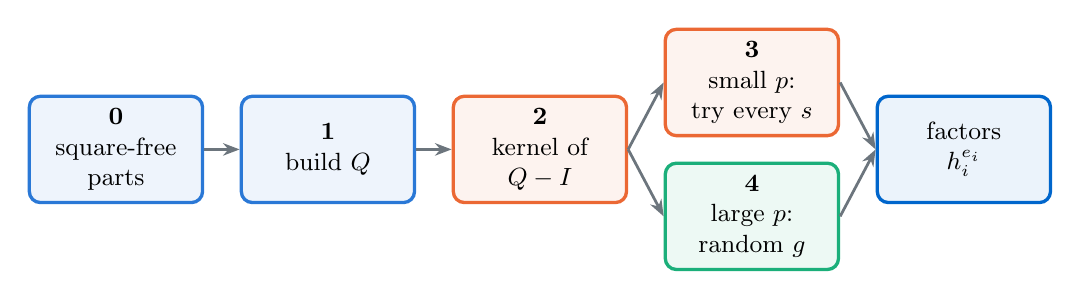
\begin{tikzpicture}
    \node[box=m1] (a) {\textbf{0}\\square-free\\parts};
    \node[box=m1, right=0.45cm of a] (b) {\textbf{1}\\build $Q$};
    \node[box=m2, right=0.45cm of b] (c) {\textbf{2}\\kernel of\\$Q - I$};
    \node[box=m2, right=0.45cm of c, yshift=0.85cm] (d) {\textbf{3}\\small $p$:\\try every $s$};
    \node[box=m3, right=0.45cm of c, yshift=-0.85cm] (e) {\textbf{4}\\large $p$:\\random $g$};
    \node[box=customblue, right=0.45cm of d, yshift=-0.85cm] (f) {factors\\$h_i^{e_i}$};
    \draw[arr] (a) -- (b); \draw[arr] (b) -- (c);
    \draw[arr] (c.east) -- (d.west); \draw[arr] (c.east) -- (e.west);
    \draw[arr] (d.east) -- (f.west); \draw[arr] (e.east) -- (f.west);
  \end{tikzpicture}
  \par\vspace{1.4em}
  {\small
  {\color{m1}\rule{0.8em}{0.8em}}~Part 1: steps 0--1\qquad
  {\color{m2}\rule{0.8em}{0.8em}}~Part 2: steps 2--3\qquad
  {\color{m3}\rule{0.8em}{0.8em}}~Part 3: step 4 and results}
  \par\vspace{0.8em}
  \aside{Sage gives us arithmetic in $\Zpx$. The matrix, the kernel and both splits are our code.}
\end{frame}

% -------------------------------------------------------------------------
\partslide{m1}{Square-free parts and $Q$}{Part 1}

\begin{frame}{Step 0: remove repeated factors first}
  Berlekamp needs $f$ \textbf{square-free}: the theorem in Part 2 counts \emph{distinct}
  factors, and $\gcd(f, g - s)$ cannot separate two copies of the same $h$.\par\medskip
  The usual tool: if $h^e \,\|\, f$ then $h^{e-1} \mid \gcd(f, f')$, so $f / \gcd(f, f')$ keeps one copy of each $h$.
  \bigskip
  \begin{block}{The trap in characteristic $p$}
    \[ (h^p)' = p\, h^{p-1} h' = 0 \]
    If $p \mid e$, all of $h^e$ stays inside $\gcd(f, f')$, and $f / \gcd(f, f')$ loses $h$ completely.
  \end{block}
  \bigskip
  Example over $\mathbb{Z}_3$: \ $(x^2 + 1)^3 = x^6 + 1$, \ $(x^6 + 1)' = 0$, \ $\gcd(f, f') = f$.
\end{frame}

\begin{frame}{Step 0: the fix is a $p$-th root}
  A polynomial with zero derivative only uses $x^0, x^p, x^{2p}, \dots$, so
  \[ \sum_j a_j\, x^{jp} = \Big(\sum_j a_j\, x^j\Big)^p \qquad \text{since } a^p = a \text{ in } \Zp \]
  \medskip
  \begin{enumerate}
    \item $c = \gcd(f, f')$, \ $w = f / c$ \ (product of $h$ with $p \nmid e$)
    \item For $k = 1, 2, \dots$: \ $y = \gcd(w, c)$; \ $w / y$ is the product of the $h$ with $p \nmid e$ and multiplicity exactly $k$; \ $w \leftarrow y$, $c \leftarrow c / y$
    \item What is left in $c$ has $c' = 0$, so it is a $p$-th power: take the root, recurse, multiply multiplicities by $p$
  \end{enumerate}
\end{frame}

\begin{frame}{Step 0 on an example}
  Over $\mathbb{Z}_5$: \quad $f = (x+1)^5\,(x^2+2)^2\,(x+3)$
  \bigskip
  \begin{center}
  \begin{tabular}{@{}lll@{}}
    \toprule
    step & computed & output \\
    \midrule
    start & $c = \gcd(f, f') = (x+1)^5 (x^2+2)$ & \\
          & $w = f/c = (x^2+2)(x+3)$ & \\
    $k = 1$ & $y = \gcd(w, c) = x^2 + 2$, \ $w / y = x + 3$ & $(x + 3,\ 1)$ \\
    $k = 2$ & $y = \gcd(w, c) = 1$, \ $w / y = x^2 + 2$ & $(x^2 + 2,\ 2)$ \\
    $p$-th root & left over $c = x^5 + 1$, \ $c' = 0$, \ root $x + 1$ & $(x + 1,\ 5)$ \\
    \bottomrule
  \end{tabular}
  \end{center}
  \bigskip
  \aside{$(x+1)^5$ never shows up in the gcd loop: its multiplicity $5$ is divisible by $p = 5$, so it stays whole inside $c$. Only the $p$-th root step finds it.}
\end{frame}

\begin{frame}{Step 1: $g \mapsto g^p$ is linear}
  In characteristic $p$:
  \[ (a + b)^p = a^p + b^p, \qquad (\lambda a)^p = \lambda a^p \text{ for } \lambda \in \Zp \]
  So for $g = \sum g_i x^i$, \quad $g^p = \sum_i g_i\, x^{ip} \equiv \sum_i g_i \cdot (x^{ip} \bmod f)$:
  a fixed combination of $d$ precomputed polynomials.
  \bigskip
  \begin{block}{The Berlekamp matrix $Q$ \quad ($d \times d$)}
    \centering row $i$ \ = \ coefficients of \ $x^{ip} \bmod f$
  \end{block}
  \bigskip
  With $v_g = (g_0, \dots, g_{d-1})$ as a row vector, \ $g^p \bmod f$ has coefficient vector $v_g\, Q$.\par
  \aside{Cost: $x^p \bmod f$ once by repeated squaring, then multiply by $x^p$ for each next row.}
\end{frame}

\begin{frame}{Step 1: $Q$ for $x^4 + 1$ over $\mathbb{Z}_3$}
  \begin{columns}[c]
    \begin{column}{0.45\textwidth}
      Using $x^4 \equiv -1$:
      \[
      \begin{array}{rcl}
        x^0 &=& 1 \\
        x^3 &=& x^3 \\
        x^6 &\equiv& 2x^2 \\
        x^9 &\equiv& x
      \end{array}
      \]
    \end{column}
    \begin{column}{0.45\textwidth}
      \[
        Q = \begin{pmatrix} 1&0&0&0 \\ 0&0&0&1 \\ 0&0&2&0 \\ 0&1&0&0 \end{pmatrix}
      \]
    \end{column}
  \end{columns}
  \bigskip
  \centering\aside{Each row is one power $x^{3i}$ written in the basis $1, x, x^2, x^3$.}
\end{frame}

% -------------------------------------------------------------------------
\partslide{m2}{The kernel and the split}{Part 2}

\begin{frame}{The idea: polynomials that behave like constants}
  \begin{itemize}
    \item $f$ irreducible: \ $\Zpx/(f)$ is a field, and the only solutions of $g^p = g$ are the constants $s \in \Zp$
    \item $f = h_1 h_2$: \ by CRT, $g$ can be a \textbf{different constant modulo each factor}, e.g.\
          $g \equiv 0 \pmod{h_1}$, \ $g \equiv 1 \pmod{h_2}$. \ Then $g^p \equiv g \pmod f$ \ and \ $\gcd(f, g) = h_1$
  \end{itemize}
  \medskip
  \begin{block}{Example over $\mathbb{Z}_3$: \ $f = x^2 + 2 = (x + 1)(x + 2)$}
    $g = 2x + 2$: \quad $g \equiv 0 \pmod{x + 1}$, \quad $g \equiv 1 \pmod{x + 2}$\par\smallskip
    $g^3 \equiv g \pmod f$, \qquad $\gcd(f, g) = x + 1$, \qquad $\gcd(f, g - 1) = x + 2$
  \end{block}
  \medskip
  \textbf{Berlekamp:} all such $g$ form a vector space $B$; find it by linear algebra, then read the factors off with gcds.
\end{frame}

\begin{frame}{Step 2: the kernel counts the factors}
  \[ B = \{\, g : \deg g < d,\ g^p \equiv g \pmod f \,\} \quad = \quad \{\, g : v_g (Q - I) = 0 \,\} \]
  \medskip
  \begin{block}{Theorem}
    If $f = h_1 \cdots h_r$ with distinct monic irreducible $h_i$, then \ $\dim B = r$.
  \end{block}
  \medskip
  We learn \textbf{how many} factors there are before finding any. \ $r = 1$ \ $\Rightarrow$ \ $f$ is irreducible.
  \medskip
  \begin{block}{How we compute $B$ (our own code, \texttt{kernel.py})}
    Gauss-Jordan on $(Q - I)^T$ over $\Zp$; each free column gives one basis vector.
    Row $0$ of $Q - I$ is zero, so the first basis vector is always $1$. Cost $O(d^3)$.
  \end{block}
\end{frame}

\begin{frame}{Why: the Chinese Remainder Theorem}
  \[
    \Zpx/(f) \;\cong\; \underbrace{\Zpx/(h_1)}_{\text{field}} \times \cdots \times \underbrace{\Zpx/(h_r)}_{\text{field}}
  \]
  \medskip
  \begin{itemize}
    \item In a field, $t^p - t$ has at most $p$ roots, and every $s \in \Zp$ is one \aside{(Fermat)}: the roots are exactly $\Zp$
    \item So $g \in B$ \ $\iff$ \ $g \equiv s_i \pmod{h_i}$ with constants $s_i \in \Zp$
    \item Any choice $(s_1, \dots, s_r) \in \Zp^r$ works: \ $B \cong \Zp^r$
  \end{itemize}
  \bigskip
  \centering{\Large $\dim B = r$}
\end{frame}

\begin{frame}{Step 3: every $g \in B$ splits $f$}
  Over $\Zp$: \quad $t^p - t = \prod_{s \in \Zp} (t - s)$
  \medskip
  \begin{block}{Split}
    \[ f \ = \prod_{s \in \Zp} \gcd(f,\ g - s) \]
  \end{block}
  \medskip
  \begin{itemize}
    \item $\gcd(f, g - s)$ collects exactly the $h_i$ with $g \equiv s_i = s \pmod{h_i}$
    \item $g$ non-constant $\Rightarrow$ not all $s_i$ equal \aside{(else $g \equiv s \bmod f$ and $\deg g < d$ force $g = s$)}, so at least two pieces
    \item For $h_i \ne h_j$ some basis vector has $s_i \ne s_j$ \aside{(if every basis vector had $s_i = s_j$, by linearity all of $B$ would, contradicting $B \cong \Zp^r$)}: refining by every basis vector finds all $r$ factors
  \end{itemize}
  \aside{We stop as soon as we hold $r$ pieces, the number the kernel told us.}
\end{frame}

\begin{frame}{Worked example: $x^4 + 1$ over $\mathbb{Z}_3$}
  \begin{columns}[T]
    \begin{column}{0.48\textwidth}
      \[
        Q - I = \begin{pmatrix} 0&0&0&0 \\ 0&2&0&1 \\ 0&0&1&0 \\ 0&1&0&2 \end{pmatrix}
      \]
      Columns $1, 2, 3$ of $v(Q-I) = 0$:\par
      $2v_1 + v_3 = 0$, \ $v_2 = 0$, \ $v_1 + 2v_3 = 0$\par
      $\Rightarrow\; v_2 = 0,\ v_3 = v_1$; \ $v_0$ free\par\medskip
      Kernel basis \ $\{\,1,\ x^3 + x\,\}$ \ $\Rightarrow$ \ $r = 2$
    \end{column}
    \begin{column}{0.48\textwidth}
      With $g = x^3 + x$:
      \[
      \begin{array}{rcl}
        \gcd(f, g - 0) &=& 1 \\
        \gcd(f, g - 1) &=& x^2 + 2x + 2 \\
        \gcd(f, g - 2) &=& x^2 + x + 2
      \end{array}
      \]
      \aside{$g \equiv 1$ mod one factor and $g \equiv 2$ mod the other: the $s_i$ of the CRT picture. No factor has $s_i = 0$.}
      \begin{block}{}
        \centering $x^4 + 1 = (x^2 + x + 2)(x^2 + 2x + 2)$
      \end{block}
    \end{column}
  \end{columns}
\end{frame}

\begin{frame}{The catch: the cost depends on $p$}
  The split tries up to \textbf{all $p$ values} of $s$, one gcd each: \quad cost $O(r\,p\,d^2)$
  \bigskip
  \begin{itemize}
    \item $p = 3$: instant
    \item Measured at $d = 30$ (12 $\to$ 14 $\to$ 16 bits: 0.023, 0.085, 0.24 s): each $4\times$ in $p$ costs $3.8\times$, then $2.8\times$. The second step is smaller because these inputs have fewer factors ($r$: $4.6 \to 3.1$); $O(r\,p)$ predicts $2.75\times$
    \item $p \approx 2^{512}$: up to $2^{512}$ gcds, never finishes
  \end{itemize}
  \bigskip
  \begin{block}{}
    Polynomial in $p$, \textbf{not} in $\log p$. So deterministic Berlekamp does not settle
    deterministic polynomial-time factoring.
  \end{block}
\end{frame}

% -------------------------------------------------------------------------
\partslide{m3}{Large $p$ and results}{Part 3}

\begin{frame}{Step 4: a random $g$ instead of every $s$}
  Pick $g = \sum_j c_j b_j$ with random $c_j \in \Zp$. Since $B \cong \Zp^r$ (CRT), the $s_i = g \bmod h_i$
  are independent and uniform in $\Zp$.
  \medskip
  \begin{block}{Euler's criterion}
    $s^{(p-1)/2} = 1$ \ exactly when $s$ is a non-zero square: \ about half of $\Zp$
  \end{block}
  \medskip
  \[ \gcd\big(f,\ g^{(p-1)/2} - 1\big) \]
  takes each $h_i$ with probability $q = \tfrac{p-1}{2p} \approx \tfrac12$, independently.
  It fails only if all $h_i$ land on the same side: probability $q^r + (1-q)^r \le \tfrac59$ for $r \ge 2$.\par
  \medskip
  \aside{Each try: $O(\log p)$ multiplications mod $f$; expected $O(\log r)$ rounds until all $r$ factors are apart.
  Polynomial in $\log p$. \quad For $p = 2$: $s_i \in \{0, 1\}$, so use $\gcd(f, g)$.}
\end{frame}

\begin{frame}{Does the coin really land half the time?}
  \begin{columns}[c]
    \begin{column}{0.5\textwidth}
      $f = h_1 h_2$ over $\mathbb{Z}_{101}$, 2000 random $g$\par\bigskip
      Split happens when exactly one coin is heads:
      \[ 2q(1-q), \quad q = \tfrac{p-1}{2p} \]
    \end{column}
    \begin{column}{0.45\textwidth}
      \centering
      {\color{muted}predicted}\par
      {\fontsize{28}{30}\selectfont\bfseries 0.500}\par\bigskip
      {\color{muted}measured}\par
      {\fontsize{28}{30}\selectfont\bfseries\color{customblue} 0.496}
    \end{column}
  \end{columns}
\end{frame}

\begin{frame}{Is it correct?}
  \begin{columns}[c]
    \begin{column}{0.32\textwidth}
      \centering
      {\fontsize{30}{32}\selectfont\bfseries\color{customblue} 500}\par
      random polynomials checked against Sage \texttt{factor()}
    \end{column}
    \begin{column}{0.32\textwidth}
      \centering
      {\fontsize{30}{32}\selectfont\bfseries\color{customblue} 378/378}\par
       benchmark outputs correct\par\aside{217 Berlekamp, 161 Cantor-Zassenhaus}
    \end{column}
    \begin{column}{0.32\textwidth}
      \centering
      {\fontsize{30}{32}\selectfont\bfseries\color{customblue} 70}\par
      tests, all passing
    \end{column}
  \end{columns}
  \bigskip\bigskip
  \centering\aside{From $p = 2$ to a 512-bit prime; multiplicities up to $p^2$; the three HW3 samples.}
\end{frame}

\begin{frame}{Berlekamp vs Cantor-Zassenhaus (from class)}
  \small
  \renewcommand{\arraystretch}{1.1}
  \begin{tabular}{@{}L{0.22\textwidth}L{0.36\textwidth}L{0.36\textwidth}@{}}
    \toprule
    & \textbf{Cantor-Zassenhaus} & \textbf{Berlekamp} \\
    \midrule
    After square-free & distinct-degree: $\gcd(f, x^{p^i} - x)$ for $i = 1, \dots, d/2$ & build $Q$, kernel of $Q - I$ \\
    Number of factors $r$ & known after distinct-degree ($\sum \deg(\text{part}) / k$) & known after one kernel: $r = \dim B$ \\
    Random $g$ & any $g \bmod f$, on a part with equal-degree factors; exponent $(p^k - 1)/2$ & $g \in B$, already a constant mod each $h_i$; exponent $(p - 1)/2$ \\
    Main cost & up to $d/2$ exponentiations by $p$ & $O(d^3)$ linear algebra, one exponentiation by $p$ \\
    Deterministic version & randomized by design & try all $s \in \Zp$: $O(p)$ \\
    \bottomrule
  \end{tabular}
  \par\medskip
  \aside{Same coin flip (Euler's criterion) at the end. Berlekamp's $g$ is already constant mod each $h_i$, so $(p-1)/2$ suffices; Cantor-Zassenhaus's $g$ is arbitrary, and $(p^k-1)/2$ maps it into $\{0, \pm 1\}$ mod each factor.}\par
\end{frame}

\begin{frame}{Berlekamp vs our HW3 Cantor-Zassenhaus: size of $p$}
  \begin{columns}[c]
    \begin{column}{0.62\textwidth}
      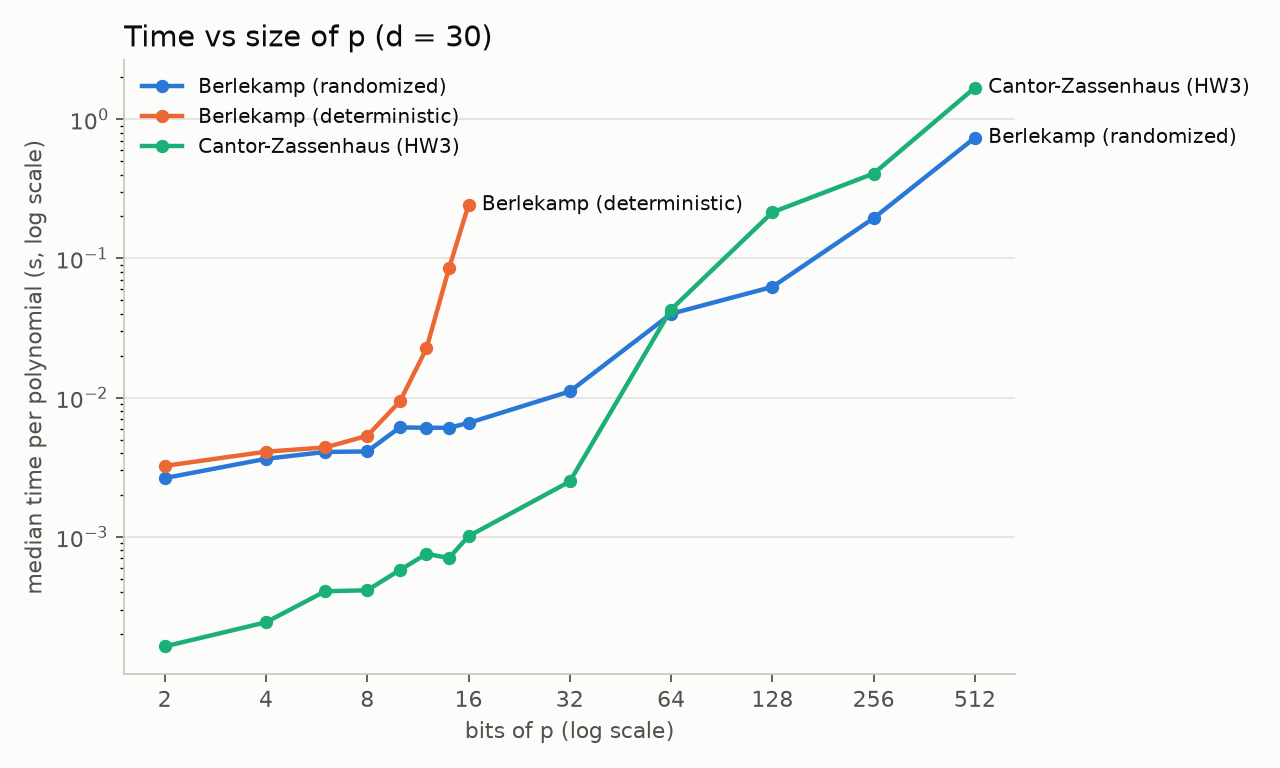
\includegraphics[width=\textwidth]{../bench/results/time_vs_p.png}
    \end{column}
    \begin{column}{0.36\textwidth}
      \small
      \begin{itemize}
        \item Deterministic grows with $p$
        \item Randomized grows with $\log p$
        \item Even at 64 bits; from 128 bits Berlekamp wins:\\
              \textbf{0.74 s vs 1.68 s} at 512 bits
      \end{itemize}
      \medskip
      \aside{Berlekamp: $x^p$ once, then a power $(p-1)/2$ per piece in $O(\log r)$ expected rounds. Cantor-Zassenhaus: up to $d/2$ powers $p$. Same inputs and library, $d = 30$.}
    \end{column}
  \end{columns}
\end{frame}

\begin{frame}{Berlekamp vs our HW3 Cantor-Zassenhaus: degree}
  \begin{columns}[c]
    \begin{column}{0.49\textwidth}
      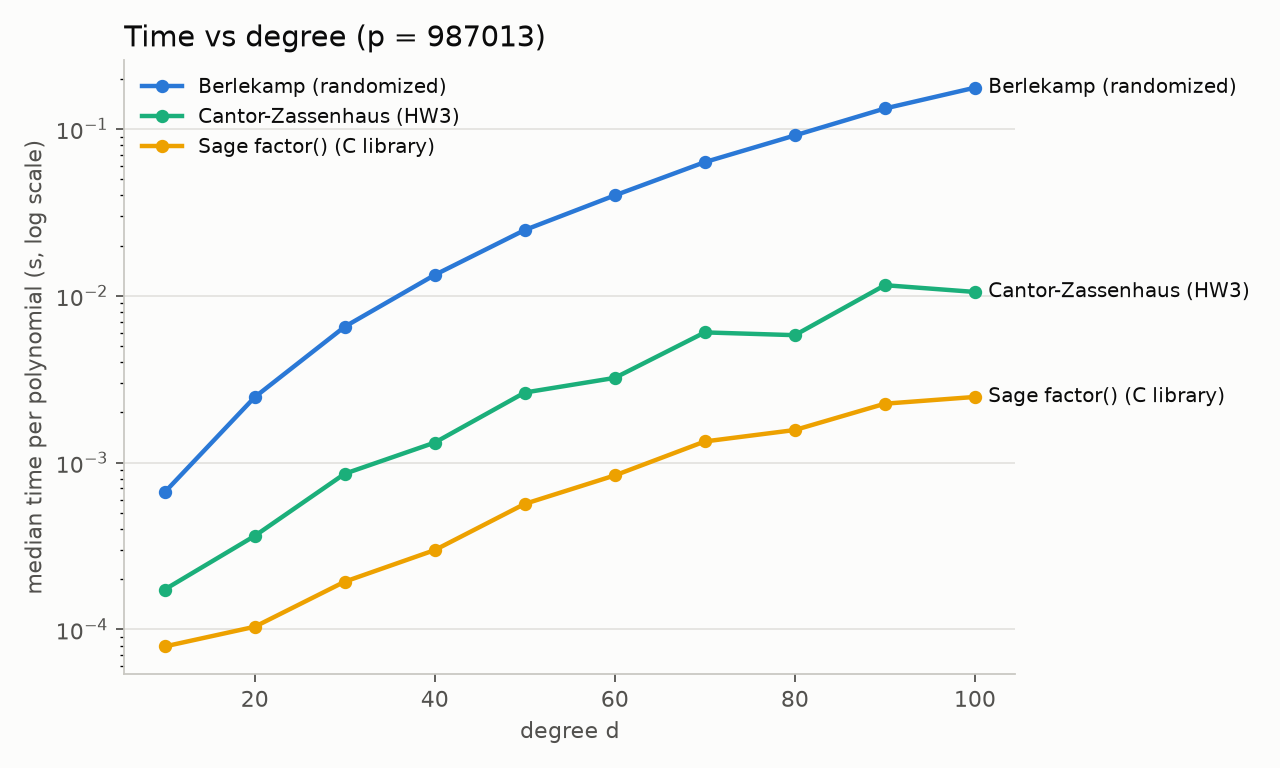
\includegraphics[width=\textwidth]{../bench/results/time_vs_degree.png}
    \end{column}
    \begin{column}{0.49\textwidth}
      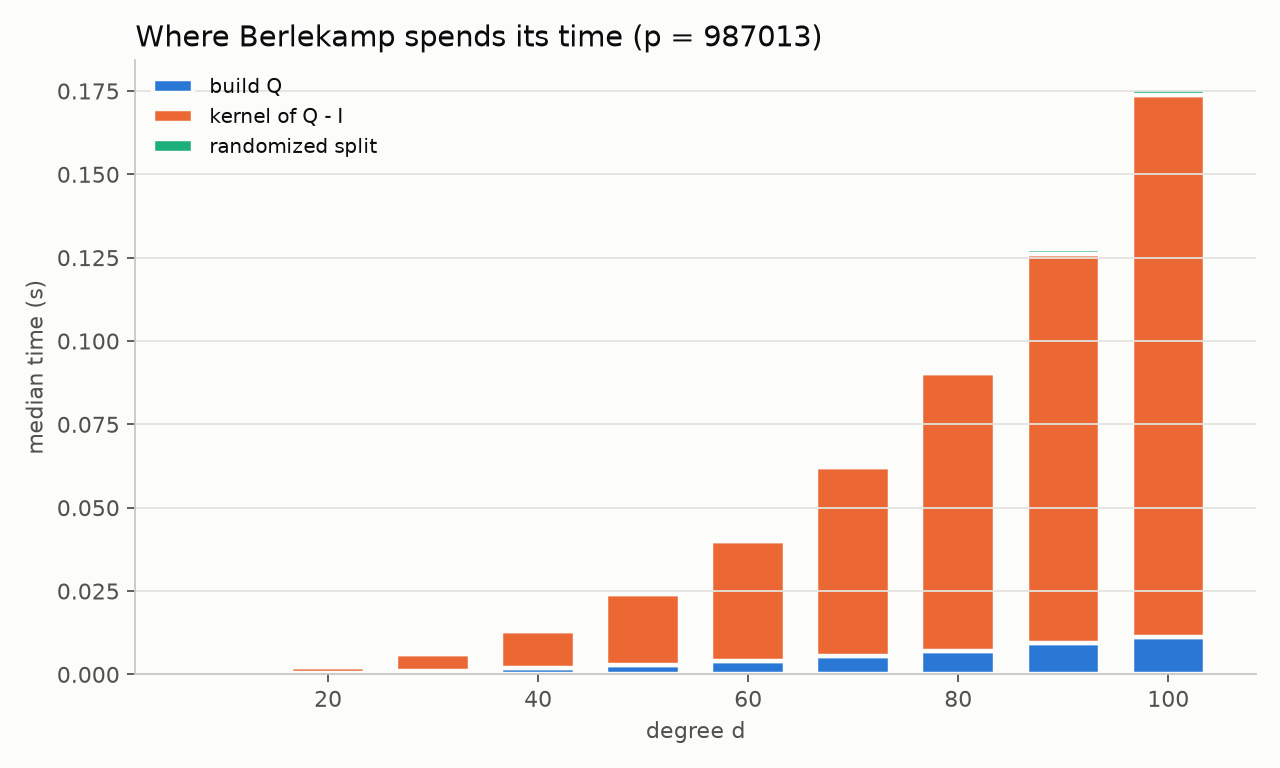
\includegraphics[width=\textwidth]{../bench/results/berlekamp_stages.png}
    \end{column}
  \end{columns}
  \medskip
  \centering
  The kernel of $Q - I$ is \textbf{over 90\%} of the time at $d = 100$: $O(d^3)$ linear algebra.\par
  \aside{Our kernel is pure-Python Gauss-Jordan; our Cantor-Zassenhaus runs on Sage's compiled C arithmetic. So at $p \approx 2^{20}$ Cantor-Zassenhaus is faster for every $d$ we measured (see ``Explaining the measurements'' for why).}
\end{frame}

\begin{frame}{Do the measurements match the theory?}
  \small
  \begin{tabular}{@{}L{0.34\textwidth}L{0.28\textwidth}L{0.32\textwidth}@{}}
    \toprule
    \textbf{Claim} & \textbf{Theory predicts} & \textbf{We measured} \\
    \midrule
    $\dim \ker(Q - I) = r$ & equals Sage's factor count & equal on every input checked \\
    $x^4 + 1 = \Phi_8$, $p$ odd: $r = 4$ iff $p \equiv 1 \pmod 8$, else $r = 2$ & $r = 4$ only for $p = 17$ among $3..23$ & $r = 4$ at $17$; $r = 2$ at $3, 5, 7, 11, 13, 19, 23$ \\
    Random split of $h_1 h_2$, $p = 101$ & $2q(1-q) = 0.500$ & $0.496$ (2000 trials) \\
    Kernel is $O(d^3)$ & $8\times$ when $d$ doubles & $7.6\times$ ($d = 50 \to 100$) \\
    Deterministic split is $O(p)$ & $4\times$ per $+2$ bits & $3.8\times$, then $2.8\times$ ($12 \to 14 \to 16$ bits; $r$ drops $4.6 \to 3.1$) \\
    Randomized split is poly$(\log p)$ & slow growth in bits & $0.003$--$0.007$ s up to 16 bits \\
    \bottomrule
  \end{tabular}
  \medskip
  \aside{Why $x^4 + 1$ behaves so: its roots are the primitive 8th roots of unity. They lie in $\Zp$ iff $8 \mid p - 1$,
  and always in $\mathbb{F}_{p^2}$ since $8 \mid p^2 - 1$ for odd $p$, so otherwise $f$ splits into two quadratics.}
\end{frame}

\begin{frame}{Explaining the measurements (1/2): size of $p$}
  \small
  \renewcommand{\arraystretch}{1.2}
  \begin{tabular}{@{}L{0.31\textwidth}L{0.65\textwidth}@{}}
    \toprule
    \textbf{What we see} & \textbf{Why} \\
    \midrule
    Deterministic split nearly flat from 2 to 8 bits ($0.003 \to 0.005$ s) &
      Building $Q$ ($O(\log p)$ multiplications) and the $O(d^3)$ kernel cost almost the same for every $p$. The $O(r\,p\,d^2)$ split only dominates from about 10 bits, then grows close to linearly in $p$. \\
    $2.8\times$, not $4\times$, from 14 to 16 bits &
      The random 16-bit inputs had fewer factors ($r$: $4.6 \to 3.1$). $O(r\,p)$ predicts $4 \times 3.1/4.6 \approx 2.75\times$. \\
    Every method jumps between 32 and 64 bits (Cantor-Zassenhaus $17\times$) &
      Sage stores $\Zpx$ with FLINT (machine words) for $p < 2^{63}$ and with NTL (multi-precision) above. A library change, not the algorithm, so we compare methods within a row. \\
    Cantor-Zassenhaus faster up to 32 bits &
      Its $d/2$ exponentiations are cheap when $\log p$ is small, while Berlekamp's kernel is a fixed $O(d^3)$ cost. From 128 bits the exponentiations dominate and Berlekamp wins. \\
    \bottomrule
  \end{tabular}
\end{frame}

\begin{frame}{Explaining the measurements (2/2): degree and probability}
  \small
  \renewcommand{\arraystretch}{1.2}
  \begin{tabular}{@{}L{0.31\textwidth}L{0.65\textwidth}@{}}
    \toprule
    \textbf{What we see} & \textbf{Why} \\
    \midrule
    Cantor-Zassenhaus $17\times$ faster at $d = 100$, $p \approx 2^{20}$ &
      Mostly constant factors: our elimination does $d^3$ Python operations, Cantor-Zassenhaus's $\approx d^2 \log d \log p$ work runs in C (FLINT). At these sizes the two bounds are of similar size. \\
    Kernel grows $7.6\times$, not $8\times$, when $d$ doubles &
      Lower-order $O(d^2)$ terms and timing noise (median of 7 runs). \\
    Coin measured $0.496$, predicted $0.500$ &
      Sampling noise: standard error $\sqrt{0.25/2000} \approx 0.011$, so the gap is $0.4$ standard errors. \\
    \bottomrule
  \end{tabular}
\end{frame}

% -------------------------------------------------------------------------
\section{Summary}

\begin{frame}{The whole algorithm and its cost}
  \begin{columns}[T]
    \begin{column}{0.56\textwidth}
      \small
      \textbf{Input} $f \in \Zpx$, \ $\deg f = d$
      \begin{enumerate}
        \item $c \leftarrow$ leading coefficient; \ make $f$ monic
        \item Square-free parts $(g, e)$ with $f = \prod g^e$
        \item For each part $g$:
          \begin{enumerate}
            \item build $Q$ \ (row $i$ = $x^{ip} \bmod g$)
            \item basis $b_1 = 1, b_2, \dots, b_r$ of $\ker(Q - I)$
            \item $r = 1$: $g$ is irreducible
            \item else split with $\gcd(g, b_j - s)$ (small $p$) or $\gcd(g, b^{(p-1)/2} - 1)$ for random $b \in B$ (large $p$) until $r$ pieces
          \end{enumerate}
        \item Output $c \cdot \prod h^e$
      \end{enumerate}
    \end{column}
    \begin{column}{0.40\textwidth}
      \small
      \begin{tabular}{@{}ll@{}}
        \toprule
        Step & Cost \\
        \midrule
        square-free & $O(d^3)$ \\
        $Q$ & $O(\log p + d)$ mults \\
        kernel & $O(d^3)$ \\
        det.\ split & $O(r\,p\,d^2)$ \\
        rand.\ split & $O(\log r \cdot \log p)$ mults$^{*}$ \\
        \bottomrule
      \end{tabular}
      \par\medskip
      \aside{mults: multiplications mod $f$. Other costs: operations in $\Zp$. $^{*}$expected.}
    \end{column}
  \end{columns}
\end{frame}

\begin{frame}{Takeaways}
  \begin{enumerate}
    \setlength{\itemsep}{0.8em}
    \item $\dim \ker(Q - I) = r$: \ Berlekamp knows the number of factors first
    \item Square-free in characteristic $p$ needs the $p$-th root step
    \item Deterministic split: polynomial in $p$, not $\log p$
    \item Randomized split: polynomial in $\log p$, beats Cantor-Zassenhaus for large $p$
    \item The bottleneck in our implementation is the $O(d^3)$ linear algebra
  \end{enumerate}
\end{frame}

\begin{frame}[plain]
  \vfill
  \centering
  {\fontsize{34}{38}\selectfont\bfseries\color{customblue} Questions?}\par\vspace{1.4em}
  \texttt{python -m kersplit --trace < examples/x4plus1\_mod3.txt}\par\vspace{0.6em}
  {\color{muted}\small Live demo: \texttt{demo.ipynb} \quad\textbullet\quad Report: \texttt{report/report.pdf}}
  \vfill
\end{frame}

\end{document}
